\begin{figure}[H]
\centerline{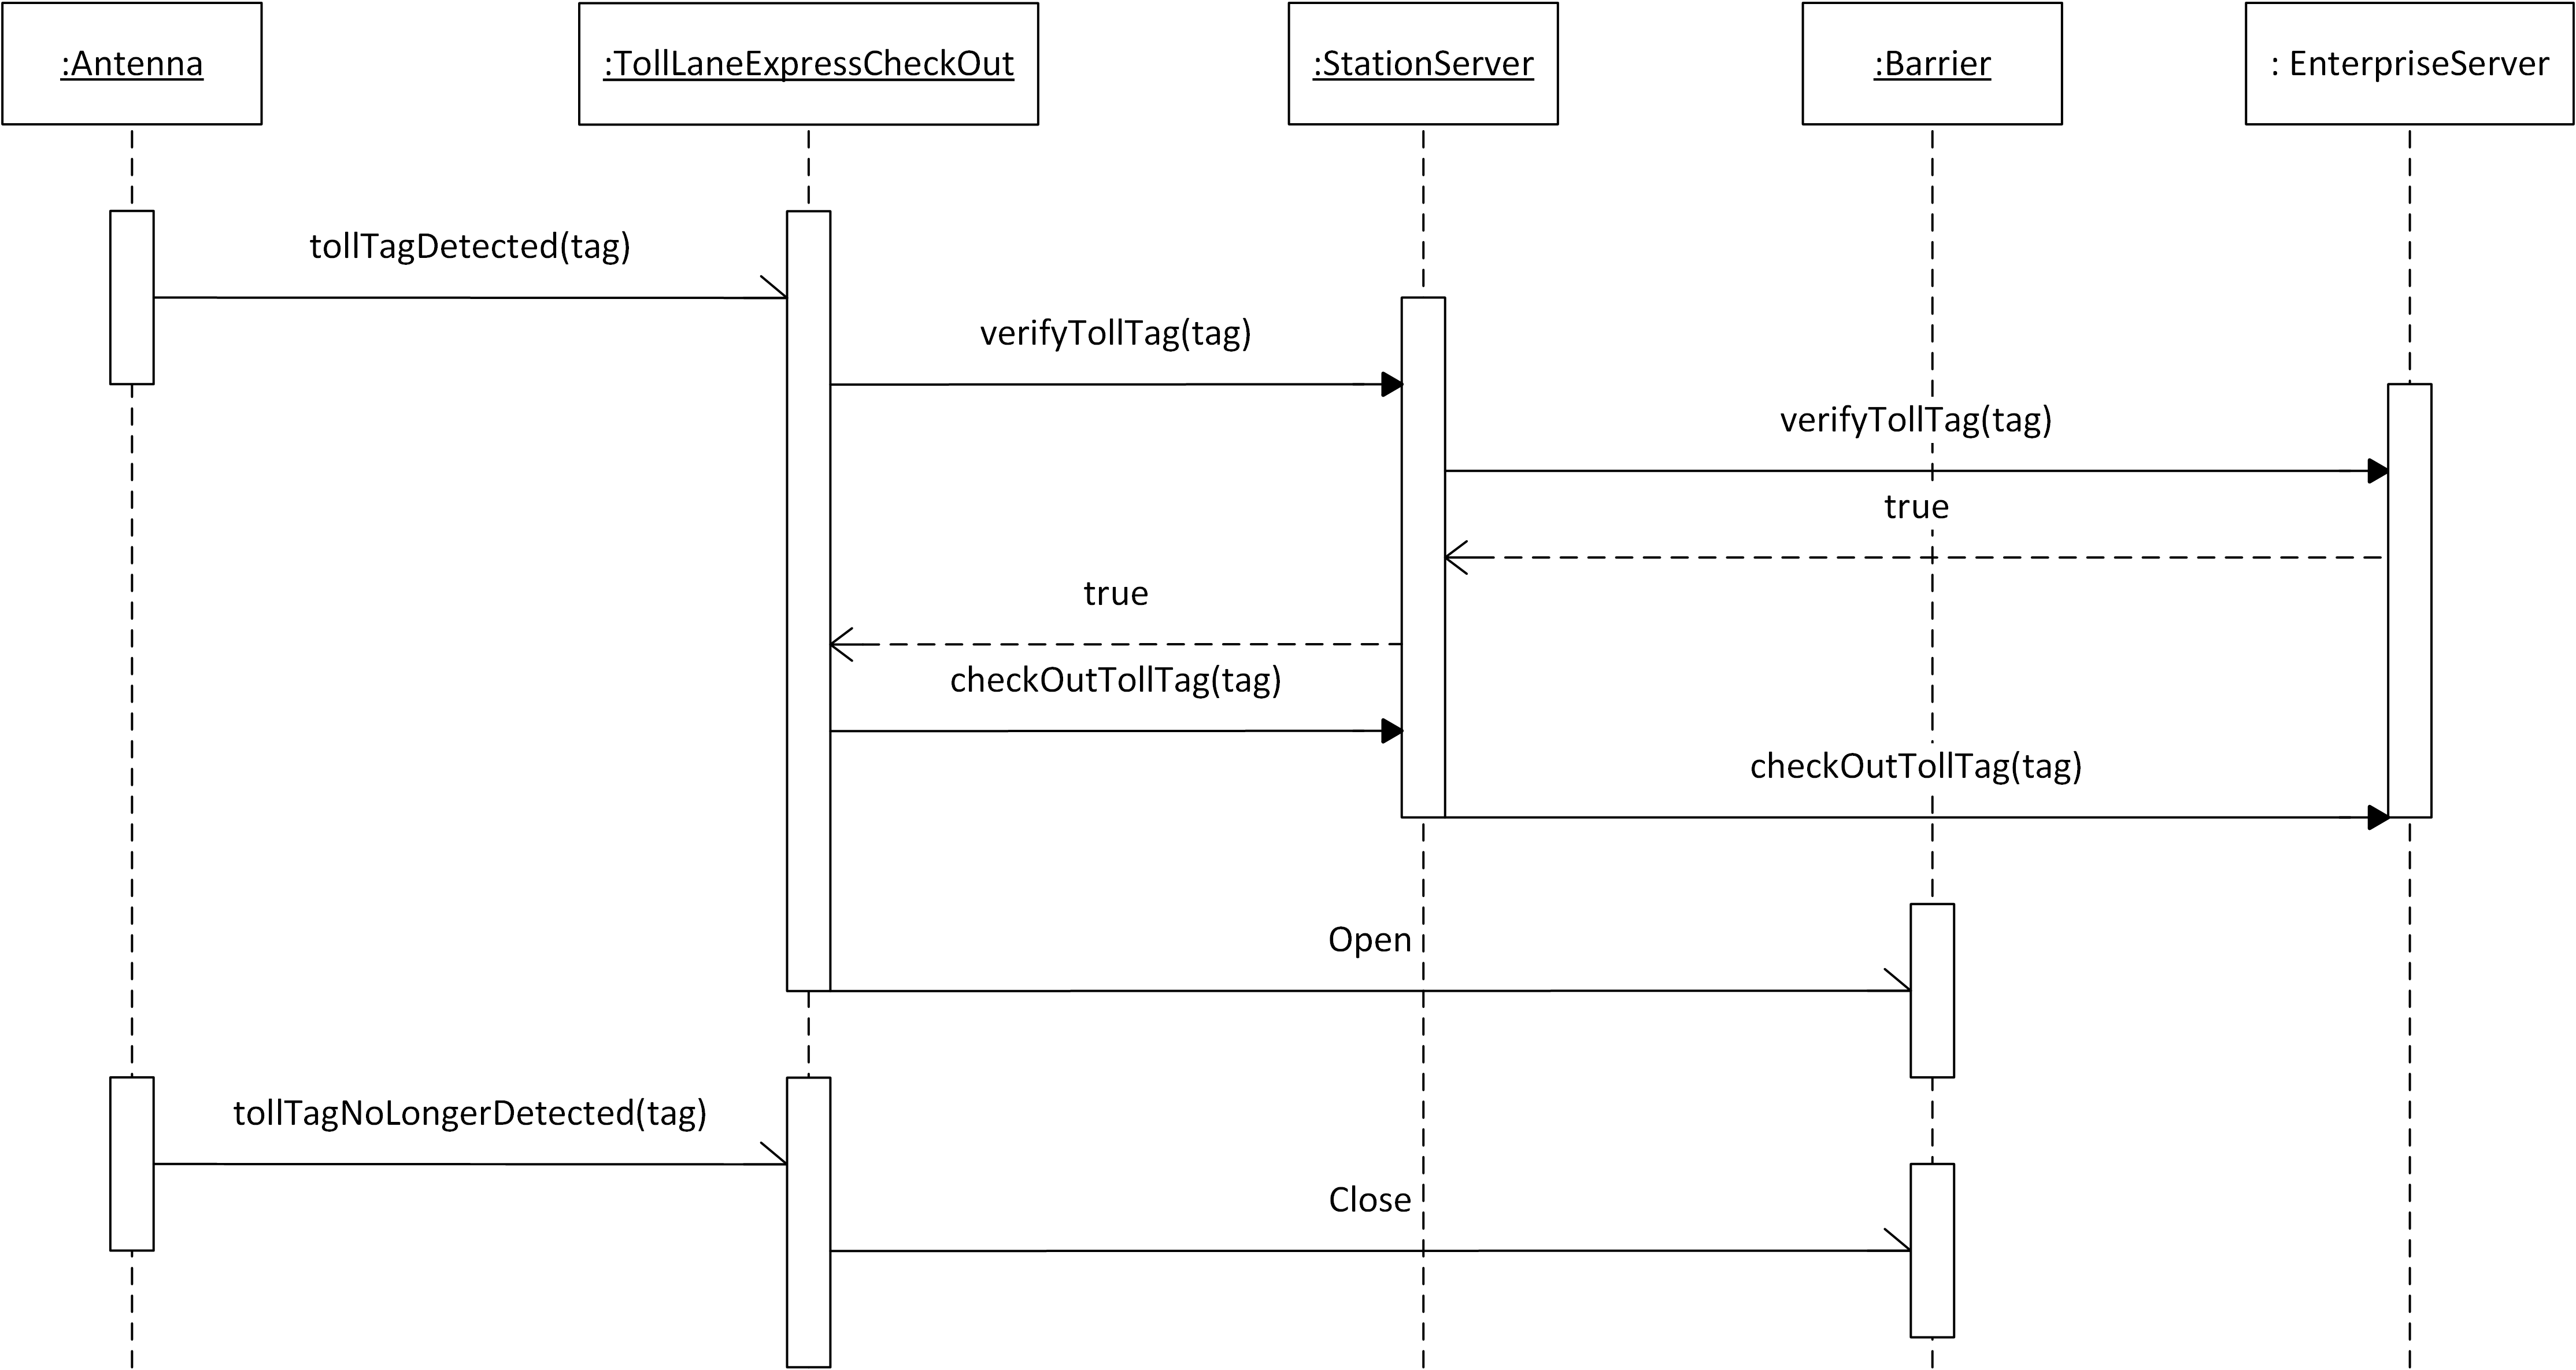
\includegraphics[width=1.4\columnwidth]{img/sequence_diagrams/sequence_diagram_toll_tag_check_out}}
\caption{Sequence diagram of toll tag check out}
\label{fig:seq_check_out_toll_tag}
\end{figure}

\begin{enumerate}
\item The customer drives up to the barrier, and awaits check out.

\begin{enumerate}
\item The lane detects the customer's toll tag through the antenna by receiving
a \texttt{tollTagDetected} message.
\end{enumerate}
\item The system checks out the customer

\begin{enumerate}
\item The lane then checks out the tag in the following manner:

\begin{enumerate}
\item It first sends \texttt{verifyTollTag} with the tag to the station server
\item The station server sends the same message to the enterprise server
\item The enterprise server then checks that the tag is checked in.
\item Once the enterprise server has verified the tag it responds with \texttt{true}
if the above condition held,
\item The station server sends the response back to the express lane.
\item When the express lane has received the response, if it was \texttt{true} it
will send a \texttt{checkOut} message which should now succeed.
\end{enumerate}
\end{enumerate}
\item The system opens the barrier.

\begin{enumerate}
\item Once the tag has been checked out, the express lane will send the
message \texttt{open} to the barrier, which will cause it to open
\end{enumerate}
\item The customer leaves the toll lane.

\begin{enumerate}
\item The lane will await the message \texttt{tollTagNoLongerDetected} from the antenna
which means the tag is no longer in range
\end{enumerate}
\item The system closes the barrier.

\begin{enumerate}
\item Once the express has received \texttt{tollTagNoLongerDetected}, it will assume
it is safe to close the barrier. It will do that by sending a \texttt{close}
message to the barrier.\end{enumerate}
\end{enumerate}

